\section{System Overview}
\label{sec:fdsp-tpcelec-overview}

\fixme{A lot of overlap with the IDR; text needs to be significantly revised for second draft, including adding more system requirements.}

%%%%%%%%%%%%%%%%%%%%%%%%%%%%%%%%%%%
\subsection{Introduction}
\label{sec:fdsp-tpcelec-overview-intro}

\fixme{I suggest that the first paragraph of this introductory section be placed under 1.1 System Overview to serve as the introduction to the section. This may require a little repharsing, but minimal changes elsewhere.}

\dword{dune} single-phase \dword{tpc} electronics hardware signal processing takes place inside the \dword{lar}, in boards that are directly mounted on the \dword{apa}; accordingly, the \dword{tpc} readout electronics are referred to as the \dword{ce}.  The electronics are mounted inside the \dword{lar} to exploit the fact that charge carrier mobility in silicon is higher and that thermal fluctuations are lower at \dword{lar} temperature than at room temperature.  For \dword{cmos} (complementary metal-oxide-semiconductor) electronics, this results in substantially higher gain and lower noise at \dword{lar} temperature than at room temperature~\cite{larCMOS}.  Mounting the front-end electronics on the \dword{apa} frames also minimizes the input capacitance.  Furthermore, placing the digitizing and multiplexing (MUX) \fixme{This abbreviation is not in the glossary.}electronics inside the cryostat reduces the total number of penetrations into the cryostat and minimizes the number of cables coming out of the cryostat.  As the full \dword{tpc} electronics chain for the \dword{spmod} includes many components on the warm side of the cryostat as well, the \dword{dune} consortium designated to organize development of this system is called the \dword{dune} \textit{Single-Phase \dword{tpc} Electronics} consortium. It is sometimes referred to as the \dword{ce} consortium for short.

The overall noise requirement drives the choice of the \dword{tpc} electronics architecture. This requirement is difficult to establish precisely, but clearly, the less electronic noise, the better the physics reach of the \dword{dune} experiment will be.  An equivalent noise charge (\dword{enc}) of less than approximately 1000$e^-$ is required for satisfactory reconstruction of accelerator neutrino interactions, but a lower noise level will yield significantly better two-track separation and primary vertex resolution, and thus higher efficiency and/or lower background for identifying electron neutrino interactions.  Setting the noise level requirement for the \dword{dune} \dword{spmod} more precisely is an ongoing effort.

The noise level enabled by having the front-end electronics in the cold (roughly half as much noise at \dword{lar} temperature than at room temperature) greatly extends the reach of the \dword{dune} physics program.  Decreasing the noise level allows measurement of smaller charge deposits , a source of risk mitigation in case the desired drift field cannot be reached or the electron lifetime in the detector is less than desired (due to the electronegative impurities in the detector). Decreasing the noise level also increases the reach of low-energy physics measurements like those associated with stellar core-collapse supernova burst neutrinos.  Finally, a low noise level allows the experiment to use low-energy $\mathrm{{}^{39}Ar}$ beta decays to calibrate the \dword{dune} \dword{spmod}.  The noise level requirement of \dword{enc}\,$<\num{1000}\,e^-$ will allow the use of $\mathrm{{}^{39}Ar}$ beta decays in calibrations at the DUNE \dword{spmod}.

To retain maximum flexibility in optimizing reconstruction algorithms after the \dword{dune} data is collected, the \dword{spmod} electronics are designed to produce a digital record representing the waveform of the current produced by charge collection/induction on the anode wires.  Each anode wire signal is input to a charge sensitive amplifier, followed by a pulse shaping circuit and an \dword{adc}.  To minimize the number of cables and cryostat penetrations, the \dwords{adc} as well as the amplifier/shapers are located in the \dword{lar}, and digitized data from many wires merge onto a much smaller set of high speed serial links.  %[Figure xx illustrates the front-end electronics architecture.  128-channel “Front-End Mother Boards” produce digitized waveforms and transmit those waveforms on four serial links through a \fdth in the top of the cryostat to “Warm Interface Boards” located in crates mounted directly on spool pieces on the outside of the cryostat. The Warm Interface Boards provide clean power and timing signals to the \dword{ce}.  All connections to the DAQ and slow control systems are made using optical fibers.] – might better cover later.

%INCLUDE AN OVERVIEW FIGURE HERE WITH THIS CAPTION:  ``Each Anode Plane Assembly (\dword{apa}) has 2560 instrumented wires.  These are read out by 20 Front-End MotherBoards (\dwords{femb}).  All cables between \dwords{femb} on a given \dword{apa} are routed through a single cryostat \fdth.  A printed circuit board connects those cables to the backplane of a Warm Electronics Interface Crate.  Warm Interface Boards mounted in this crate receive data from the \dwords{femb} and transmit it to the data acquisition system.''

%%%%%%%%%%%%%%%%%%%%%%%%%%%%%%%%%%%
\subsection{Design Considerations}
\label{sec:fdsp-tpcelec-overview-design}

The \dword{ce} signal processing is implemented in application-specific integrated circuits (\dwords{asic})
using \dword{cmos} technology.  The \dword{ce} is continuously read out, resulting in a digitized \dword{adc}
sample from each \dword{apa} channel (wire) up to every \SI{500}{ns} (\SI{{\sim}2}{MHz} sampling rate).

Each individual \dword{apa} has \num{2560} channels read out by \num{20} \dfirsts{femb}, with
each \dshort{femb} enabling digitized wire readout from \num{128} channels.  One cable bundle connects each \dshort{femb} to
the outside of the cryostat via a \dword{ce} signal cable flange located at the \dword{ce} \fdth at the
top of the cryostat, where a single flange services each \dword{apa}, as shown in Figure~\ref{fig:connections}.  Two \dword{ce} signal flanges are on each \fdth and together account for all electronics channels associated with a pair of \dword{apa}s (upper and lower, vertically arranged).
Each cable bundle contains wires for low-voltage (\dword{lv}) power, high-speed data readout, and
clock or digital-control signal distribution.  Eight separate cables carry the \dword{tpc} wire bias voltages
from the signal flange to the \dword{apa} wire bias boards, in addition to the bias voltages for the field
cage termination electrodes and for the electron diverters.  An additional flange on the top of each \fdth services the \dword{pds} cables associated with the \dword{apa} pair.

\begin{dunefigure}
[Connections between the signal flanges and \dword{apa}]
{fig:connections}
{Connections between the signal flanges and \dword{apa}. The lower \dword{apa} shares the photon detector flange with the upper \dword{apa} but has a separate TPC readout flange. A \textit{\dword{ce} module} consists of all \dword{ce} associated with \num{128} channels of digitized readout.}
%\hspace{1cm}
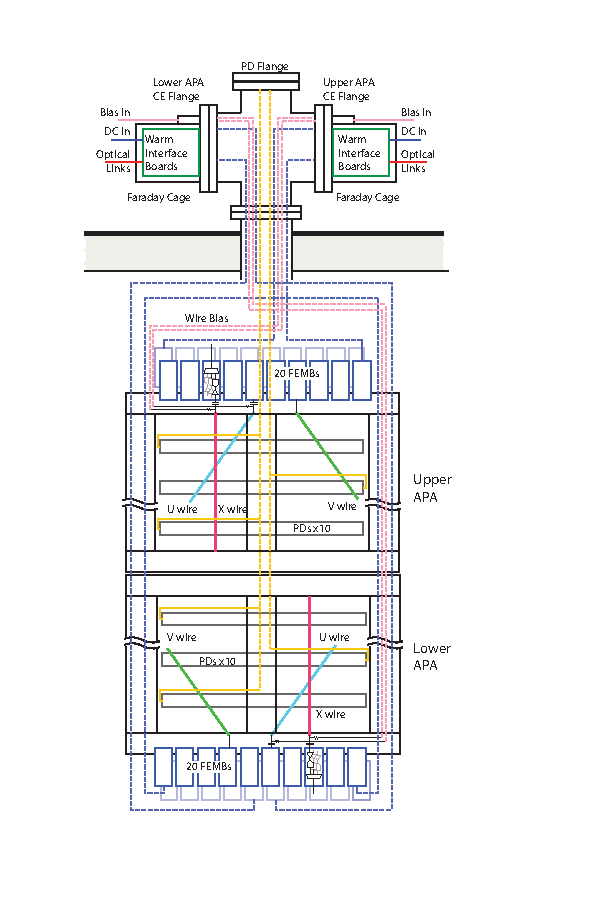
\includegraphics[width=0.7\textwidth]{sp-tpcelec-DUNE-FD-APA-readout-scheme-v1.pdf}
\end{dunefigure}

The components of the \dword{ce} system are the following:
\begin{itemize}
\item{\dwords{femb}, on which the \dwords{asic} are mounted, and which are installed on the \dword{apa}s;}
\item{cables for the data, clock, and control signals; \dword{lv} power; and wire bias voltages between the \dword{apa} and the signal flanges (cold cables);}
\item{signal flanges with a \dword{ce} \fdth to pass the data, clock, and control signals; \dword{lv} power; and \dword{apa} wire-bias voltages between the inside and outside of the cryostat; and the corresponding cryostat penetrations and spool pieces;}
\item{%warm interface electronics crates (
\dwords{wiec} mounted on the signal flanges and contain
the %warm interface boards (
\dwords{wib} and %power and timing cards (
\dwords{ptc} for further processing
and distribution of the signals entering and exiting the cryostat;}
%\item{fiber cables for transmitting data and clock/control signals between the \dwords{wiec} and the
%data acquisition (DAQ) and slow control systems;}
\item{cables for \dword{lv} power and wire bias voltages between the signal flange and external power
supplies (warm cables); and}
\item{\dword{lv} power supplies for the \dword{ce} and bias-voltage power supplies for the \dword{apa}s.}
\end{itemize}

Table~\ref{tab:elecNums} lists the component type, the quantity required for each type, and the number of channels per component of each type.

\begin{dunetable}
[TPC electronics components and quantities for a single \dword{apa} of a %the DUNE \single 
\dword{spmod}.]
{llr}
{tab:elecNums}
{TPC electronics components and quantities for a single \dword{apa} of the DUNE \dword{spmod}.}
\textbf{Element} &\textbf{Quantity} & \textbf{Channels per element}\\ \toprowrule
Front-end mother board (\dword{femb}) & \num{20} per \dword{apa} & \num{128} \\ \colhline
FE \dword{asic} chip & \num{8} per \dword{femb} & \num{16} \\ \colhline
\dword{adc} \dword{asic} chip & \num{8} per \dword{femb} & \num{16} \\ \colhline
\dword{coldata} \dword{asic} chip & \num{2} per \dword{femb} & \num{64} \\ \colhline
Cold cable bundle & \num{1} per \dword{femb} & \num{128} \\ \colhline
Signal flange & \num{1} per \dword{apa} & \num{2560} \\ \colhline
\dword{ce} \fdth & \num{1} per \dword{apa} pair & \num{2560} \\ \colhline
Warm interface board (\dword{wib}) & \num{5} per \dword{apa} & \num{512} \\ \colhline
Warm interface electronics crate (\dword{wiec}) & \num{1} per \dword{apa} & \num{2560} \\ \colhline
Power and timing card (\dword{ptc}) & \num{1} per \dword{apa} & \num{2560} \\ \colhline
Power and timing backplane (PTB) & \num{1} per \dword{apa} & \num{2560} \\
%\dword{lv} power mainframe & ? & ? \\ \colhline
%\dword{lv} supply module & ? & ? \\ \colhline
%wire bias mini-crate & ? & ? \\ \colhline
%wire bias supply module & ? & ? \\
\end{dunetable}

The baseline design for the \dword{spmod} TPC electronics calls for three types of \dwords{asic} inside  the \dword{lar}:
\begin{itemize}
\item{a \num{16}-channel \dword{fe} \dword{asic} for amplification and pulse shaping (referred to as \dword{larasic});}
\item{a \num{16}-channel \num{12}-bit \dword{adc} \dword{asic} operating at \SI{{\sim}2}{MHz}; and}
\item{a \num{64}-channel control and communications \dword{asic} (referred to as \dword{coldata}).}
\end{itemize}

The \dword{fe} \dword{asic} has been prototyped and is close to meeting requirements (discussed in Section~\ref{sec:fdsp-tpcelec-overview-scope}). Another prototype to address issues in the version deployed in \dword{pdsp} should be finished in early 2019. Key portions of the control and communications \dword{asic} (also called the \dword{coldata} \dword{asic}) have been prototyped and meet requirements.  However, we have determined that the BNL-designed P1-\dword{adc} \dword{asic} now being used in \dword{pdsp} does not meet requirements, and accordingly, its development has been terminated.  A new \dword{adc} \dword{asic} (also called the cold \dword{adc} \dword{asic}) is being developed by an LBNL-\fnal-BNL collaboration; first prototypes should be ready in February 2019.  The first full prototype of the controls and communication \dword{asic} should also be available for testing in June 2019.

To maximize the probability of quickly developing a complete design for cold TPC \dword{fe} electronics, an alternative solution is also being investigated: a single \num{64}-channel \dword{asic} that will consolidate all three functions listed above.  This design is being done at SLAC, and the first prototypes will be tested in February 2019.  An \dword{adc} solution in the form of a commercial, off-the-shelf (COTS) option serves as an additional backup option and has already been tested; this option will be explored further if the other two \dword{adc} solutions being considered do not meet the requirements for \dword{dune}.

While the higher charge carrier mobility at \dword{lar} temperature than at room temperature is central to improving the performance of \dword{ce}, it also leads to the \textit{hot carrier effect}.  In n-type MOS \fixme{This abbreviation is not in the glossary.} transistors, the carriers (electrons) can acquire enough kinetic energy to ionize silicon in the active channel.  This charge can become trapped and lead to effects (including threshold shifts) similar to those caused by radiation damage.  This effect can cause MOS circuits to age much more quickly at \dword{lar} temperature than at room temperature, reducing performance and potentially causing failure.  To mitigate this effect, the maximum \efield in transistor channels must be lower than the field that can be reliably used at room temperature.  This is accomplished by using transistors fabricated longer than is typical and operated at reduced bias voltage.  Any commercial circuits used in the \dword{lar} must be carefully tested to ensure they will perform well for the expected \num{20}-year lifetime of \dword{dune}; reliability studies for front-end electronics designs in consideration are discussed in Section~\ref{sec:fdsp-tpcelec-qa-reliability}.

A series of tests are planned to demonstrate that the \dword{ce} system design will meet \dword{dune} requirements. These include two system tests: one using the \dword{pdsp} \textit{cold box} at CERN and one using a new small \dword{lartpc} at \fnal. The latter will also accommodate one half-length \dword{dune} \dword{pd} and will provide a low-noise environment that will allow detailed comparisons of the performance of the new \dwords{asic}. It will also enable the study of interactions between the \dword{tpc} readout and other systems, including the \dword{pd} readout and the \dword{hv} distribution. These test facilities are discussed in more detail in Section~\ref{sec:fdsp-tpcelec-qa-facilities}. A second period of data taking is also planned for the \dword{pdsp} detector, with final \dword{apa}s including the final \dwords{asic} and \dwords{femb} replacing the current prototypes. This second run of \dword{pdsp} is planned for 2021-2022.

\fixme{Update on second ProtoDUNE run?  Also discuss more what can be done with current ProtoDUNE run}

%%%%%%%%%%%%%%%%%%%%%%%%%%%%%%%%%%%
\subsection{Scope and Requirements}
\label{sec:fdsp-tpcelec-overview-scope}

In addition to the noise requirement (less than \num{1000}\,$e^{-}$), several additional requirements determine most of the other important \dword{tpc} electronics specifications:  

\begin{itemize}
\item{The \dword{fe} peaking time must  %should 
be  in the range \numrange{1}{3}\,\si{\micro\second}.  This requirement derives primarily from the time required for drifting charges to travel from one plane of anode wires to the next.}
\item{The \dword{fe} must %should 
 have an adjustable baseline.  In other words, the signal from induction wires is bipolar while the signal from  collection wires is mostly unipolar.}
\item{The \dword{adc} sampling frequency must %should 
be \SI{{\sim}2}{MHz}.  This value is chosen to match a \dword{fe} shaping time of \SI{1}{\micro\second} (approximate Nyquist condition) while minimizing the data rate.}
\item{The system must have a linear response up to an impulse input of at least \num{500000}\,$e^{-}$.  This roughly corresponds to the largest ionization signals expected in events where multiple protons are produced in the primary event vertex, in particular, when the trajectories of one or more of those particles are parallel to the wire, causing the charge over a long path length to be collected within a short time.}
\item{The \dword{adc} must not contribute significantly to overall \dword{fe} noise. This requirement depends on the gain of the \dword{fe} but for each gain setting, translates into requirements on \dword{adc} parameters, including non-linearity and noise.}
\item{The \dword{adc} must digitize the charge deposited on the wires with 12~bits of precision.  The lower end of the \dword{adc} dynamic range is driven by the requirement that the ADC digitization does not contribute to total electronics noise. The upper end of the \dword{adc} dynamic range is defined by the previous requirement for the signal saturation level. Combining these two requirements with the specification for the total electronics noise results in the need for 12~bits digitization.}
\item{The power dissipated by the electronics located in the \dword{lar} must 
be less than \SI{50}{mW/channel}.  Lower power dissipation is desirable because the mass of the power cables scales with  power.  Ongoing studies focus on whether the amount of power dissipated by the electronics should be minimized further because of potential complications from argon boiling; in principle, this should not be a problem because the \dword{ce} boxes housing the \dwords{femb} are designed to channel bubbles to the \dword{apa} frames.}
\end{itemize}

Finally, all electronics in the \dword{lar} must 
be highly reliable because accessing the \dword{ce} for repair is not possible once the cryostat is filled with \dword{lar}. Ongoing studies are quantifying the effect of failures in the \dword{tpc} and electronics, including single wire failures and failures of groups of \num{16}, \num{64}, or \num{128} channels.

\fixme{Will add in formal top-level requirements that have already been included Doc DB 11074 (eight associated with TPC Electronics); Anne will advise how/where to integrate into chapter}

%%%%%%%%%%%%%%%%%%%%%%%%%%%%%%%%%%%
\subsection{ProtoDUNE-SP Results}
\label{sec:fdsp-tpcelec-overview-pdune}

\fixme{A discussion of ProtoDUNE studies that the CE consortium needs should be discussed at an upcoming CE consortium meeting; this discussion and subsequent plans will inform the updating of this section for the second draft}

The Single Phase \dword{protodune}-\dword{sp} detector, described in Chapter~\ref{ch:sp-execsum}, is a 700~ton fiducial volume \dword{lartpc} with 15,360 sense wires that are read out by the \dword{ce} system described in Section~\ref{sec:fdsp-tpcelec-qa-facilities-pdune}. The system was deployed in a beam line of the CERN Neutrino Platform in 2018 and continues to take cosmic event data into 2019. The goal of the \dword{protodune}-\dword{sp} \dword{tpc} readout was to validate the concept and the design of the integrated \dword{apa}+\dword{ce} readout and measure the performance of the \dword{ce} system with components as close as possible to the final \dword{dune} \dword{tpc} readout.

Each of the six \dword{protodune}-\dword{sp} \dword{apa}+\dword{ce} readout units consists of 2,560 sense wires, of which 960 are 6.0~meter long collection wires and 1,600 are 7.4~meter \fixme{Do these measurements of the wires need to be in LATEX code?} long induction wires. Each one was tested in a full scale cold box in cold gaseous Nitrogen (GN2) with a complete \dword{ce} readout system identical to the one on the detector before installation in the cryostat. Figure~\ref{fig:apa2-cycle} shows the \dword{enc}, which is the charge in electrons that would have to arrive at the sense wires to generate a signal with the RMS \fixme{RMS is not in the glossary.} measured by the front end electronics as a function of cold cycle time. At a stable temperature of 160 Kelvin, \fixme{Should Kelvin be abbreviated?} the \dword{enc} for all three wire planes is less than 500~e$^-$.

\begin{dunefigure}
[\dword{pdsp} APA2 noise levels measured in GN2 at CERN Cold Box]
{fig:apa2-cycle}
{Left Y-axis: ENC (in electrons) for U, V, and X (red, blue, and green curves) sense wire planes as a function of time (hours) for the APA2 cold cycle in GN2 in the CERN Cold Box; right Y-axis: temperature (orange curve) measured at the level of the front-end electronics.}
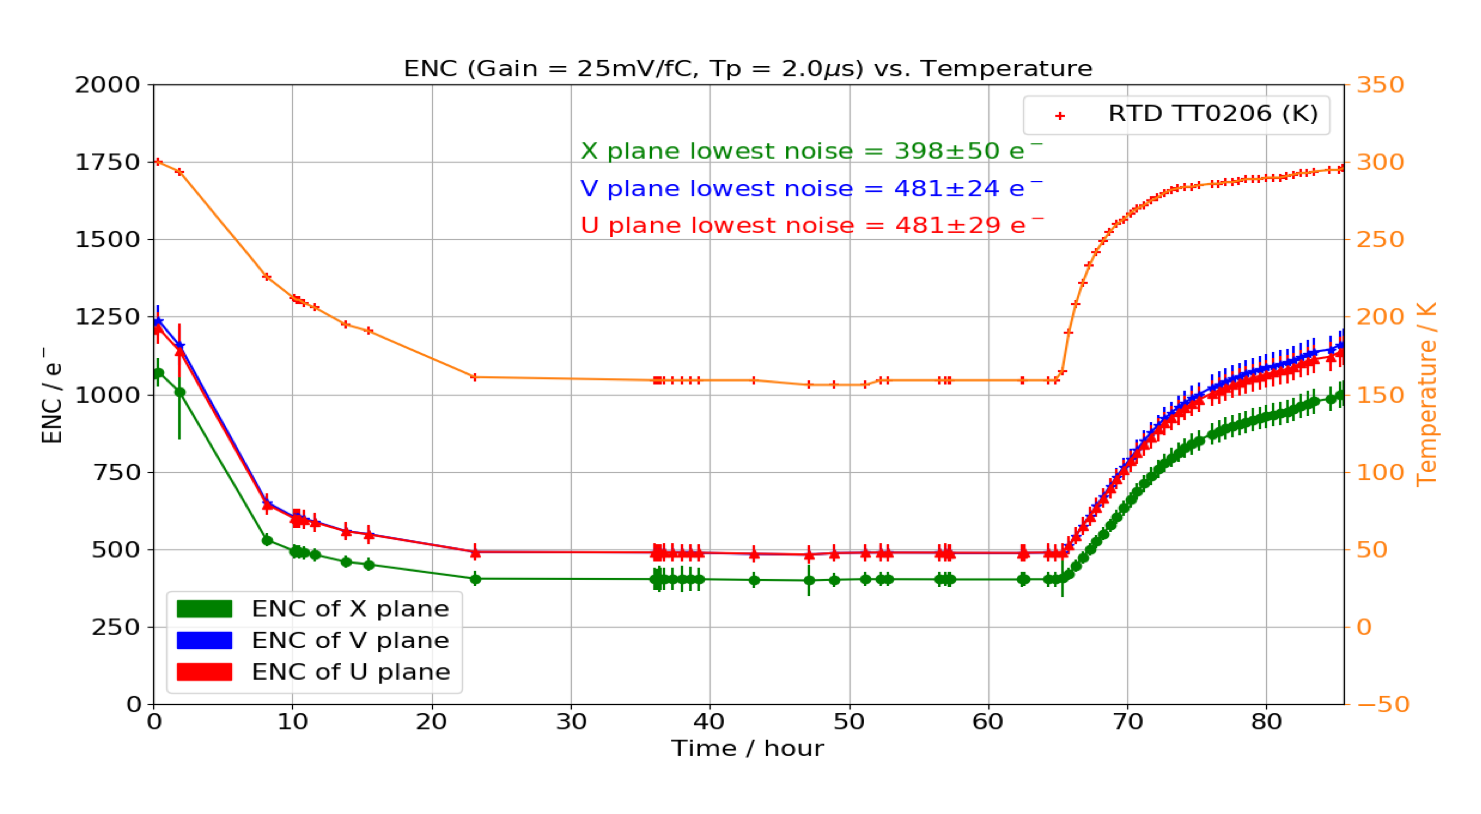
\includegraphics[width=1.0\linewidth]{sp-tpcelec-apa2.png}
\end{dunefigure}

After the cryostat was filled with \dword{lar} and the drift and wire bias HV were set to nominal (defined in Chapter~\ref{ch:sp-execsum}), 99.7\% of the \dword{tpc} readout channels were alive. The following channels were expected to be unresponsive to charge deposited on the wires:
\begin{itemize}
\item Four electronics channels, suggesting a dead channel in the electronics, all on collection wires on three different \dwords{apa};
\item $\sim$35 channels measured with  consistent with no capacitive load on the \dword{fe} electronics, suggesting an open connection somewhere in front of the \dword{ce} system, scattered randomly throughout the detector and on all wire planes.
\end{itemize}
With the detector in nominal operating conditions, the \dword{enc} was approximately 550~e$^-$ on the collection wires and approximately 750~e$^-$ averaged over all operational channels. Figure~\ref{fig:apa3-noise} shows the \dword{enc} in electrons for all channels of one of the \dword{apa}+\dword{ce} readout units. The collection channels with \dword{enc}$>$1500~e$^-$ are caused by an artifact in the generation of cold \dword{adc} \dword{asic} used in \dword{protodune}-\dword{sp}. The channels in all three planes with \dword{enc}$<$300~e$^-$ have an open connection somewhere in front of the \dword{ce} system.

\begin{dunefigure}
[TPC noise levels measured at \dword{pdsp} after \lar fill]
{fig:apa3-noise}
{ENC (in electrons) for all U, V, and X (red, blue, and green curves) sense wire planes for one ProtoDUNE APA with the detector in nominal operating conditions.}
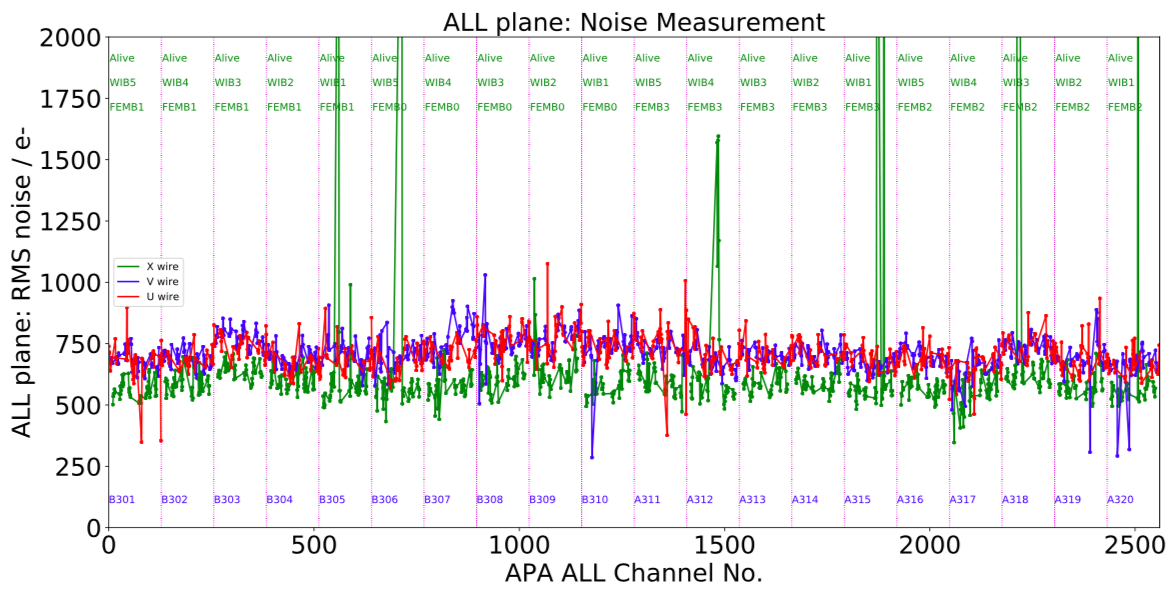
\includegraphics[width=1.0\linewidth]{sp-tpcelec-apa3-enc.png}
\end{dunefigure}

The overall performance of the \dword{ce} system in \dword{protodune}-\dword{sp} satisfies the \dword{dune} single phase \dword{fd} \dword{ce} system requirements listed in Section~\ref{sec:fdsp-tpcelec-overview-scope}. The overall system architecture, described in Section~\ref{sec:fdsp-tpcelec-overview-design}, will remain the same for the \dword{dune} \dword{ce}. However, several improvements and updates to the \dword{ce} system design were motivated by the results of the testing and commissioning of, and the data-taking with, the \dword{protodune}-\dword{sp} electronics. They will be discussed in this chapter.

\fixme{Should show noise levels for all APAs in Figure~\ref{fig:apa3-noise}, not just APA 3...}
